\documentclass{book}

\usepackage{amssymb}
\usepackage{amsmath}
\usepackage{amsthm}
\usepackage{arydshln}
\usepackage{calc}
\usepackage{cancel}
\usepackage{caption}
\usepackage{cite}
\usepackage{color}
\usepackage{enumitem}
\usepackage{esint}
\usepackage{etoolbox}
\usepackage{float}
\usepackage{framed}
\usepackage{fullpage}
\usepackage{gensymb}
\usepackage[margin=1in]{geometry}
\usepackage{graphicx}
\usepackage{listings}
\usepackage{multirow}
\usepackage{subfiles}
\usepackage{rsfso}
\usepackage{tikz}
\usepackage{tikz-3dplot}
\usepackage{ushort}
\usepackage{wrapfig}
\usepackage{xcolor}
\usepackage{soul}
\usepackage{epstopdf}
\usepackage{array}
\usepackage{slashbox}

% pdf versions
\pdfoptionpdfminorversion=7

% handle page stretching
\raggedbottom

% Graphics file location
\graphicspath{{Graphics/}{../Graphics/}}

% Use for drawings
\usetikzlibrary{angles,arrows,calc,decorations,intersections,patterns,positioning,quotes,shapes}
\usetikzlibrary{shapes.geometric}
\usetikzlibrary{decorations.pathreplacing}
\newcommand{\midarrow}{\tikz \draw[-latex] (0,0) -- +(.1,0);}

% Tikz commands for drawing block diagrams, etc...
\tikzset{%
	block/.style    = {draw, rectangle, minimum height = 2em, minimum width = 2em},
	sum/.style      = {draw, circle}, % Adder
	input/.style    = {fill=white, rectangle}, % Input
	output/.style   = {fill=white, rectangle}, % Output
	waypoint/.style   = {coordinate}, % Output
}

\tikzset{%
	startstop/.style= {draw, rectangle, rounded corners, minimum width=2cm, minimum height=1cm,text centered},
	inout/.style    = {draw, trapezium, trapezium left angle=70, trapezium right angle=110, minimum width=2cm, minimum height=1cm, text centered},
	process/.style  = {draw, rectangle, minimum width=2cm, minimum height=1cm, text centered},
	decision/.style = {draw, diamond, minimum width=1.5cm, minimum height=1cm, text centered, diamond, aspect=2},
	arrow/.style    = {thick,-latex,>=stealth},		
}

\tikzset{
	saveuse path/.code 2 args={
		\pgfkeysalso{#1/.style={insert path={#2}}}%
		\global\expandafter\let\csname pgfk@\pgfkeyscurrentpath/.@cmd\expandafter\endcsname
		% not optimal as it is now global through out the document
		\csname pgfk@\pgfkeyscurrentpath/.@cmd\endcsname
		\pgfkeysalso{#1}},
	/pgf/math set seed/.code=\pgfmathsetseed{#1}}

% Define Laplace, Fourier transform symbols
\newcommand{\LT}{\mathcal{L}}
\newcommand{\FT}{\mathcal{F}}

% Define adjugate function
\newcommand{\adj}{\text{adj}}

% Define rank function
\newcommand{\rank}{\text{rank}}

% commands to speed up writing j\omega and s-plane
\newcommand{\jw}{j\omega}
\newcommand{\jt}{j\theta}
\newcommand{\wt}{\omega t}
\newcommand{\spl}{s\textrm{-plane}}
\newcommand{\Lm}{\textrm{Lm }}
% Clean up overline/underline for math mode
\def\obar#1{\bar{#1}}
\def\ubar#1{\ushort{#1}}

\newcommand{\exmp}{\subsubsection*{Example}}
\newcommand{\nib}{\noindent$ \bullet\ $}


\begin{document}
\chapter*{Lecture 9}
Last time: Block Diagram Algebra
\begin{itemize}
	\item Basic Elements
	\item Interconnections
	\item Basic Forms
	\item Block Diagram Manipulation
\end{itemize}

This lecture will be concerned with issues of accuracy of the final value of a system's output, in other words how close a system's final value is to the desired value. Another name for this is \textbf{steady-state error}.

A control system design is usually evaluated by looking at the systems performance in \textbf{at least} three areas:
\begin{itemize}
	\item Transient response
	\item Stability
	\item Steady-state response
\end{itemize}

\begin{center}
	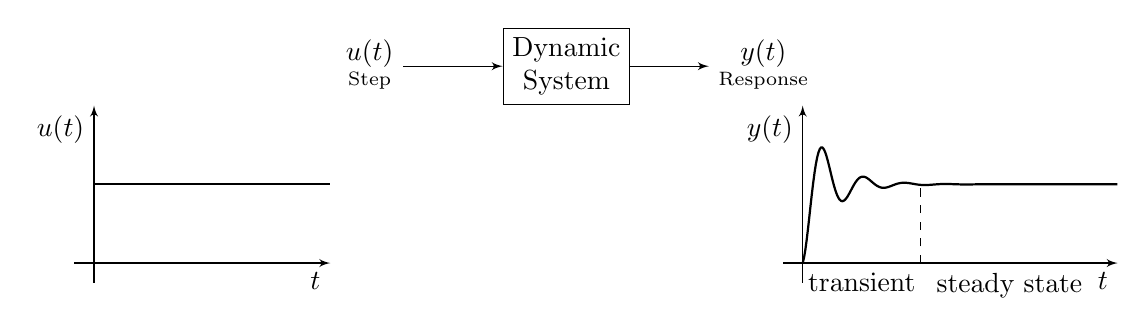
\begin{tikzpicture}[node distance=2.5cm,auto,>=latex']
	\node [input, align=center] (U) {$\underset{\text{Step}}{u(t)}$};
	\node [block, align=center] (G) [right of=U] {Dynamic\\System};
	\node [output, align=center] (y) [right of=G] {$\underset{\text{Response}}{y(t)}$};
	\draw[->] (U) -- node {} (G);
	\draw[->] (G) -- node {} (y);
	
	\begin{scope}[shift={(-3.5cm,-2.5cm)}]
	\draw[->] (-0.25,0) -- (3,0) node[below left] {$ t $};  % x Axis
	\draw[->] (0,-0.25) -- (0,2) node[below left] {$ u(t) $};  % y Axis
	\draw[thick] (0,1) -- (3,1);
	\end{scope}
	
	
	\begin{scope}[shift={(5.5cm,-2.5cm)}]
	\draw[->] (-0.25,0) -- (4,0) node[below left] {$ t $};  % x Axis
	\draw[->] (0,-0.25) -- (0,2) node[below left] {$ y(t) $};  % y Axis
	
	\draw[thick,domain=0:4,samples=240] plot (\x,{1-exp(-3*\x)*cos((180/pi)*12*\x)});
	\draw [dashed] (1.5,0) -- (1.5,1);
	\node[below] at (0.75,0) {transient};
	\node[below] at (2.625,0) {steady state};
	\end{scope}
	\end{tikzpicture}
\end{center}

We have covered transient response characteristics for step inputs of 1st and 2nd order systems, and we have covered stability. Now, we want to discuss steady-state behavior. The key quantity used to evaluate the steady-state behavior is its \textbf{steady-state error}.

Steady-state error is the difference between input and output as $ t\to\infty $. It tells you how well a system can follow a given command. Steady-state behavior of a system can vary depending on the command, $ r(t) $. Consider the following input signals:

\begin{center}
	\begin{tabular}{ m{1.5cm} m{3.5cm} m{4.25cm} }
		Step & \begin{tikzpicture}
		\draw[->] (-0.25,0) -- (3,0) node[below left] {$ t $};  % x Axis
		\draw[->] (0,-0.25) -- (0,2) node[below left] {$ u(t) $};  % y Axis
		\draw[thick] (0,1) -- (3,1);
		\end{tikzpicture} & \begin{minipage}{0.25\textwidth}\[ r(t) = 1(t) \] \[ R(s) = \frac{1}{s} \] 	\vspace{2em}	\end{minipage} \\
		
		Ramp & 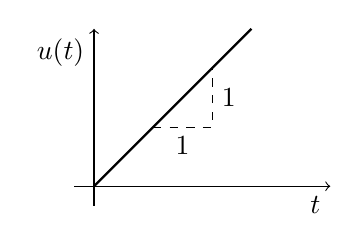
\begin{tikzpicture}
		\draw[->] (-0.25,0) -- (3,0) node[below left] {$ t $};  % x Axis
		\draw[->] (0,-0.25) -- (0,2) node[below left] {$ u(t) $};  % y Axis
		\draw[thick] (0,0) -- (2,2);
		\draw[dashed] (0.75,0.75) -- node[below,pos=0.5] {1} (1.5,0.75) -- node[right,pos=0.5] {1} (1.5,1.5);
		\end{tikzpicture} & \begin{minipage}{0.25\textwidth}\[ r(t) = t\cdot1(t) \] \[ R(s) = \frac{1}{s^2} \] 	\vspace{2em}	\end{minipage} \\
		
		Parabola & 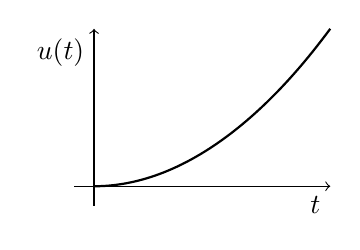
\begin{tikzpicture}
		\draw[->] (-0.25,0) -- (3,0) node[below left] {$ t $};  % x Axis
		\draw[->] (0,-0.25) -- (0,2) node[below left] {$ u(t) $};  % y Axis
		\draw[thick] (0,0) parabola (3,2);
		\end{tikzpicture} & \begin{minipage}{0.25\textwidth}\[ r(t) = t^2\cdot 1(t) \] \[ R(s) = \frac{1}{s^3} \] 	\vspace{2em}	\end{minipage} \\
	\end{tabular}
\end{center}

Let's look at some examples of steady-state error:
\begin{center}
	\begin{tikzpicture}[scale=1.625]
	\begin{scope}
	\draw[->] (-0.25,0) -- (3,0) node[below left] {$ t $};  % x Axis
	\draw[->] (0,-0.25) -- (0,2) node[below left] {};  % y Axis
	\draw[domain=0:3,samples=500] plot (\x,{1.35-1.35*exp(-3*\x)});
	\draw[dashed] (0,1.5) node[left] {}-- (3,1.5);
	\draw[-latex] (2.5,1.5+1/3) node[left] {$ e_{ss} $} -- (2.5,1.5);
	\draw[-latex] (2.5,1.35-1/3) -- (2.5,1.35);
	\end{scope}
	
	\begin{scope}[shift={(4.5cm,0cm)}]
	\draw[->] (-0.25,0) -- (3,0) node[below left] {$ t $};  % x Axis
	\draw[->] (0,-0.25) -- (0,2) node[below left] {$ y(t) $};  % y Axis
	\draw[domain=0:3,samples=500] plot (\x,{(1/2)+(-1/2)*exp(-\x) + (-1/2-1/2)*\x*exp(-\x) + (1/2)*\x});
	\draw[dashed] (0,0) -- (3,1.5) node[right] {$ u(t) $};
	\draw[-latex] (2.75,1.65+1/3) node[left] {$ e_{ss} $} -- (2.75,1.65);
	\draw[-latex] (2.75,2.75/2-1/3) -- (2.75,2.75/2);
	\end{scope}
	
	\begin{scope}[shift={(0cm,-3cm)}]
	\draw[->] (-0.25,0) -- (3,0) node[below left] {$ t $};  % x Axis
	\draw[->] (0,-0.25) -- (0,2) node[below left] {$ y(t) $};  % y Axis
	\draw[domain=0:3,samples=500] plot (\x,{-1/3 + 1/3*exp(-2*\x) + (2/3)*\x});
	\draw[dashed] (0,0) -- (3,2) node[right] {$ u(t) $};
	\draw[-latex] (2,5/3) node[above] {$ e_{ss} $} -- (2,4/3);
	\draw[-latex] (2,2/3) -- (2,1);
	\end{scope}
	
	\begin{scope}[shift={(4.5cm,-3cm)}]
	\draw[->] (-0.25,0) -- (3,0) node[below left] {$ t $};  % x Axis
	\draw[->] (0,-0.25) -- (0,2) node[below left] {$ y(t) $};  % y Axis
	\draw (0,0) parabola (3,1.25) node[right] {$ e_{ss} = \infty $};
	\draw[dashed] (0,0) parabola (3,2) node[right] {$ u(t) $};
	\end{scope}
	\end{tikzpicture}
\end{center}
How do we find the steady-state error?
\begin{enumerate}
	\item Find an expression of $ E(s) $
	\item Verify that $e(t) $ has a final value (check stability, etc...)
	\item Apply the Final Value Theorem
\end{enumerate}

\exmp
Consider this unity feedback system:
\begin{center}
	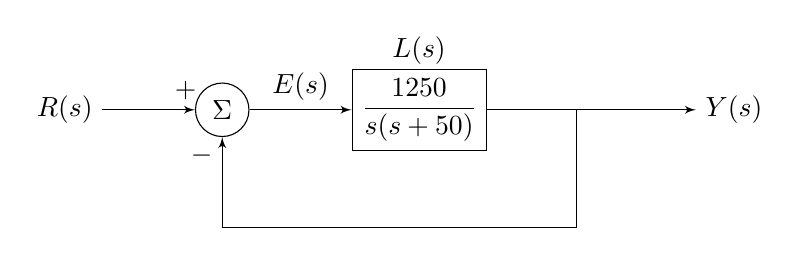
\begin{tikzpicture}[node distance=2.0cm,auto,>=latex']
	\node [input,align=center] (r) {$ R(s) $};
	\node [sum] (sumr) [right of=r] {$\Sigma$};
	\node [block] (gc) [right of=sumr,node distance=2.5cm] {$ \dfrac{1250}{s(s+50)} $};
	\node [waypoint] (sumd) [right of=gc] {};
	\node [output,align=center] (y) [right of=sumd]{$ Y(s) $};
	\node [waypoint] (h) [below of=gc,node distance=1.5cm] {};
	
	\draw[->] (r) -- node[pos=0.9] {$+$} (sumr);
	\draw[->] (sumr) -- node {$E(s)$} (gc);
	\draw[->] (gc) -- (y);
	\draw[->] (sumd) |- (h)-| node[pos=0.9] {$-$} (sumr);
	\node[above of=gc,node distance=0.75cm] {$ L(s) $};
	\end{tikzpicture}
\end{center}
What is the steady-state error for an input of $ r(t) = 5t1(t) $?In this case,
\[ E(s) = R(s) - Y(s) \]
where
\begin{align*}
Y(s) & = L(s)E(s) = L(s)\times (R(s)-Y(s)) \\
Y(s) & = L(s)R(s) - L(s)Y(s) \\
Y(s) + L(s)Y(s) & = L(s)R(s) \\
\Rightarrow \quad Y(s) & = \frac{L(s)}{1+L(s)}R(s)
\end{align*}
So, 
\[ E(s) = R(s) - \frac{L(s)}{1+L(s)}R(s) = \frac{1}{1+L(s)}R(s). \]
Substituting in the given $ L(s) $ and $ R(s) = \LT[r(t)] = 5/s^2 $,
\[ E(s) = \frac{1}{1+\dfrac{1250}{s(s+50)}}\cdot\frac{5}{s^2} = \frac{s(s+50)}{s(s+50)+1250}\cdot\frac{5}{s^2} \]
Then, apply the Final Value Theorem $ \left(e_{ss} = \lim\limits_{s\to 0} s\cdot E(s) \right) $:
\[ s\cdot E(s) = \frac{5(s+50)}{s^2+50s+1250} \]
\[ e_{ss} = \lim_{s\to0} \frac{5(s+50)}{s^2+50s+1250} = \frac{5\cdot50}{1250} = 0.2 \]

Next, we will look at more general treatment of steady-state error for \textbf{unity feedback systems}. Let's start with some definitions.
\paragraph*{System Type} The system type of a closed-loop system with unity feedback is the number of poles of the system's open-loop transfer function ($ L $) located at the origin of the system.
\exmp
\begin{center}
	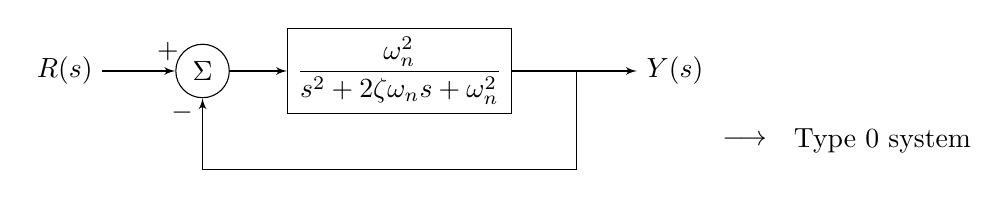
\begin{tikzpicture}[node distance=1.75cm,auto,>=latex']
	\node [input,align=center] (r) {$ R(s) $};
	\node [sum] (sumr) [right of=r] {$\Sigma$};
	\node [block] (gc) [right of=sumr,node distance=2.5cm] {$ \dfrac{\omega_n^2}{s^2+2\zeta\omega_ns + \omega_n^2} $};
	\node [waypoint] (sumd) [right of=gc,node distance=2.25cm] {};
	\node [output,align=center] (y) [right of=sumd,node distance=1.25cm]{$ Y(s) $};
	\node [waypoint] (h) [below of=gc,node distance=1.25cm] {};
	
	\draw[->] (r) -- node[pos=0.9] {$+$} (sumr);
	\draw[->] (sumr) -- (gc);
	\draw[->] (gc) -- (y);
	\draw[->] (sumd) |- (h)-| node[pos=0.9] {$-$} (sumr);
	
	\node[below right of = y,node distance=1.25cm] (ta) {$ \longrightarrow $};
	\node[right of = ta] {Type 0 system};
	\end{tikzpicture}
\end{center}
\begin{center}
	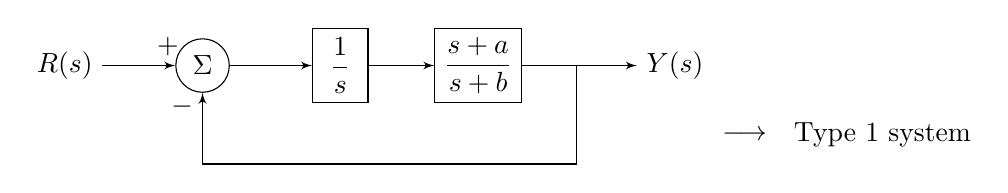
\begin{tikzpicture}[node distance=1.75cm,auto,>=latex']
	\node [input,align=center] (r) {$ R(s) $};
	\node [sum] (sumr) [right of=r] {$\Sigma$};
	\node [block] (gc) [right of=sumr] {$ \dfrac{1}{s} $};
	\node [block] (gp) [right of=gc] {$ \dfrac{s+a}{s+b} $};
	\node [waypoint] (sumd) [right of=gp,node distance=1.25cm] {};
	\node [output,align=center] (y) [right of=sumd,node distance=1.25cm]{$ Y(s) $};
	\node [waypoint] (h) [below of=gc,node distance=1.25cm] {};
	
	\draw[->] (r) -- node[pos=0.9] {$+$} (sumr);
	\draw[->] (sumr) --  (gc);
	\draw[->] (gc) -- (gp);
	\draw[->] (gp) -- (y);
	\draw[->] (sumd) |- (h)-| node[pos=0.9] {$-$} (sumr);
	
	\node[below right of = y,node distance=1.25cm] (ta) {$ \longrightarrow $};
	\node[right of = ta] {Type 1 system};
	\end{tikzpicture}
\end{center}
\begin{center}
	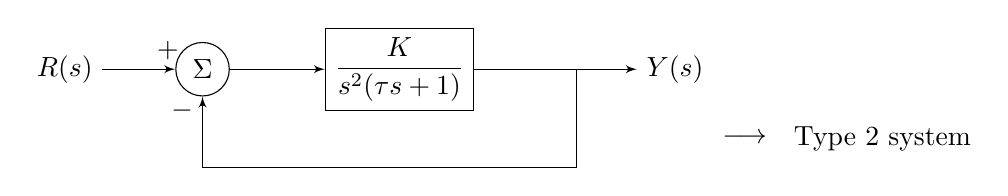
\begin{tikzpicture}[node distance=1.75cm,auto,>=latex']
	\node [input,align=center] (r) {$ R(s) $};
	\node [sum] (sumr) [right of=r] {$\Sigma$};
	\node [block] (gc) [right of=sumr,node distance=2.5cm] {$ \dfrac{K}{s^2(\tau s+1)} $};
	\node [waypoint] (sumd) [right of=gc,node distance=2.25cm] {};
	\node [output,align=center] (y) [right of=sumd,node distance=1.25cm]{$ Y(s) $};
	\node [waypoint] (h) [below of=gc,node distance=1.25cm] {};
	
	\draw[->] (r) -- node[pos=0.9] {$+$} (sumr);
	\draw[->] (sumr) -- (gc);
	\draw[->] (gc) -- (y);
	\draw[->] (sumd) |- (h)-| node[pos=0.9] {$-$} (sumr);
	
	\node[below right of = y,node distance=1.25cm] (ta) {$ \longrightarrow $};
	\node[right of = ta] {Type 2 system};
	\end{tikzpicture}
\end{center}
\[ \text{etc}\ldots \]

We want to consider the steady-state error for unity feedback systems produced by different \textbf{systems types} in response to different \textbf{test signals}.
\begin{center}
	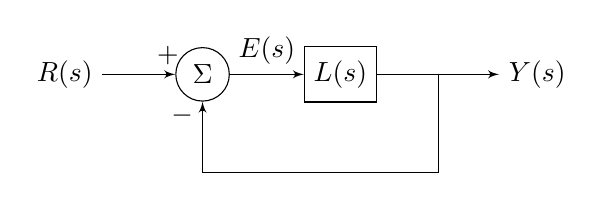
\begin{tikzpicture}[node distance=1.75cm,auto,>=latex']
	\node [input,align=center] (r) {$ R(s) $};
	\node [sum] (sumr) [right of=r] {$\Sigma$};
	\node [block] (gc) [right of=sumr] {$ L(s) $};
	\node [waypoint] (sumd) [right of=gc,node distance=1.25cm] {};
	\node [output,align=center] (y) [right of=sumd,node distance=1.25cm]{$ Y(s) $};
	\node [waypoint] (h) [below of=gc,node distance=1.25cm] {};
	
	\draw[->] (r) -- node[pos=0.9] {$+$} (sumr);
	\draw[->] (sumr) -- node[above] {$E(s)$} (gc);
	\draw[->] (gc) -- (y);
	\draw[->] (sumd) |- (h)-| node[pos=0.9] {$-$} (sumr);
	\end{tikzpicture}
\end{center}
$ L(s) $ can always be written as
\[ L(s) = \frac{K(b_ms^m + b_{m-1}s^{m-1} + \ldots+b_1s+1)}{s^p(a_ns^n + a_{n-1}s^{n-1} + \ldots+a_1s+1)} = \frac{Kb(s)}{s^pa(s)} \]
Note that the system type is equal to $ p $ here, $ p \geq 0 $ and $ p \leq 2 $.

Next we can consider some test signal $ R(s) = \dfrac{1}{s^q} $, where $ q $ here is $ \geq 1 $ and $ \leq 3 $. So,
\begin{align*}
E(s) & = R(s) - Y(s)\\
& = \frac{1}{1+L(s)}R(s)\\
& = \frac{1}{1+K\dfrac{b(s)}{s^pa(s)}}\cdot\frac{1}{s^q}\\
& = \frac{s^pa(s)}{s^q(s^pa(s)+Kb(s))}
\end{align*}
Then, apply the Final Value Theorem:
\[ e_{ss} = sE(s)\big|_{s=0} = \left. \frac{s^{p+1}a(s)}{s^q(s^pa(s)+Kb(s))}\right|_{s=0}   \]
At $ s=0 $, $ a(0)=b(0)=1 $. So,
\[ e_{ss} = \left. \frac{s^{p+1}}{s^q(s^p+K)}\right|_{s=0} = \left. \frac{s^{p-q+1}}{s^p+K}\right|_{s=0}   \]
We now have a general expression for steady-state error for different system and input types. How can we use this? Consider some possible system types and test signals:
\begin{center}
	\begin{tabular}{ccc|c|c l}
		& & \multicolumn{3}{ c }{System Type} & \\ \noalign{\smallskip}  
		& \multicolumn{1}{ c| }{} & $ p=0 $ & $ p=1 $ & $ p=2 $ & \\ \cline{2-5} \noalign{\smallskip}
		\multicolumn{1}{ c  }{\multirow{3}{*}{Powers} } & \multicolumn{1}{ c| }{Unit Step $ q=1 $} & $ \dfrac{1}{1+K_p} $ & $ \begin{array}{c}0 \\ {(K_p=\infty)}	\end{array} $ & $ \begin{array}{c}0 \\ {(K_p=\infty)}	\end{array} $ & where $ K=K_p $ when $ p=0 $ \\ \cline{2-5} \noalign{\smallskip}
		\multicolumn{1}{ c  }{} & 	\multicolumn{1}{ c| }{Unit Ramp $ q=2 $} & $ \begin{array}{c}\infty \\ {(K_v=0)}	\end{array} $ & $ \dfrac{1}{K_v} $ & $ \begin{array}{c}0 \\ {(K_v=\infty)}	\end{array} $ & where $ K=K_v $ when $ p=1 $ \\ \cline{2-5} \noalign{\smallskip}
		\multicolumn{1}{ c  }{} &  \multicolumn{1}{ c| }{Unit Parabola $ q=3 $} & $ \begin{array}{c}\infty \\ {(K_a=0)}	\end{array} $ & $ \begin{array}{c}\infty \\ {(K_a=0)}	\end{array} $ & $ \dfrac{1}{K_a} $ & where $ K=K_a $ when $ p=2 $ \\  \noalign{\smallskip}
	\end{tabular}
\end{center}
To distinguish between these, the $ K $ in the case of Type 0 systems is called the ``position error constant'' $ K_p $, the $ K $ in the case of Type 1 systems is called the ``velocity error constant'' $ K_v $, and the $ K $ in the case of Type 2 systems is called the ``acceleration error constant'' $ K_a $. 

How do we find these values? Recall what $ K $ is: We wrote $ L(s) $ as
\[ L(s) = \frac{K(b_ms^m + b_{m-1}s^{m-1} + \ldots+b_1s+1)}{s^p(a_ns^n + a_{n-1}s^{n-1} + \ldots+a_1s+1)} = \frac{Kb(s)}{s^pa(s)} \]
For steady state error ($ t\to \infty $) we are interested in $ L(s) $ as $ s\to 0 $. By the above definition of $ L(s) $: as $ s\to 0 $, $ a(s)=b(s)= 1 $ leaving us with $ K/s^p $. In other words. 
\[ \text{For }p=0,\quad L(s) = \frac{Kb(s)}{a(s)} \quad\Rightarrow\quad \lim_{s\to0}L(s) = \frac{Kb(0)}{a(0)} = \frac{K\cdot1}{1} = K \equiv K_p \]
The derivations of $ K_v $ and $ K_p $ are not given here, but follow a similar process. In summary:
\begin{align*}
\text{Type 0 ($ p=0 $): }K_p&=L(0)\text{ or }\lim_{s\to0}L(s)\\
\text{Type 1 ($ p=1 $): }K_v&=\lim\limits_{s\to0}sL(s)\\
\text{Type 2 ($ p=2 $): }K_a&=\lim\limits_{s\to0}s^2L(s)
\end{align*}

\exmp
Ramp Input:
\begin{center}
		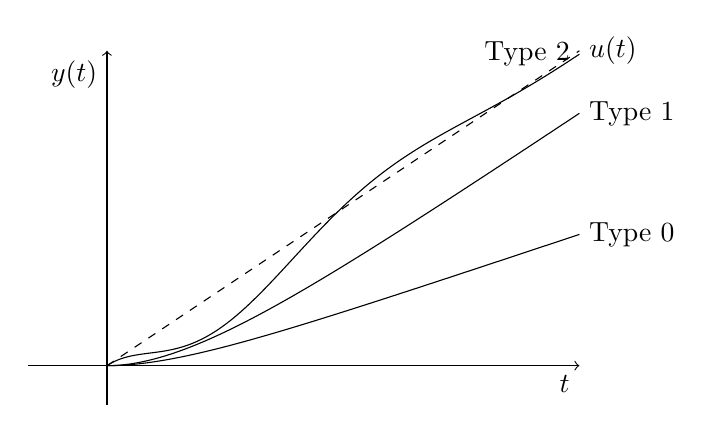
\begin{tikzpicture}[scale=2]
	\draw[->] (-0.5,0) -- (3,0) node[below left] {$ t $};  % x Axis
	\draw[->] (0,-0.25) -- (0,2) node[below left] {$ y(t) $};  % y Axis
	\draw[domain=0:3,samples=500] plot (\x,{-2/5 + 2/5*exp(-(5/3)*\x) + (2/3)*\x}) node[right] {Type 1};
	\draw[domain=0:3,samples=500] plot (\x,{-1/6 + 1/6*exp(-2*\x) + (1/3)*\x}) node[right] {Type 0};
	
	\draw[domain=0:3,samples=500] plot (\x,{ (3/16)*e^(-\x)*( -sqrt(2)*sin((180/pi)*\x*sqrt(8)) + 2*cos((180/pi)*\x*sqrt(8)) - 2*e^(-2*\x) ) + (2/3)*\x}) node[left] {Type 2};
	\draw[dashed] (0,0) -- (3,2) node[right] {$ u(t) $};
	\end{tikzpicture}
\end{center}
Steady-state error going to $ \infty $ (for the Type 0 system) doesn't mean that we are unstable. Rather, it means the system is incapable of ramping up fast enough to follow the ramp input. For the Type 2 system, $ e_{ss}\to0 $ points towards high gain. 

\exmp
Problem 7.1 from the book.
\begin{center}
	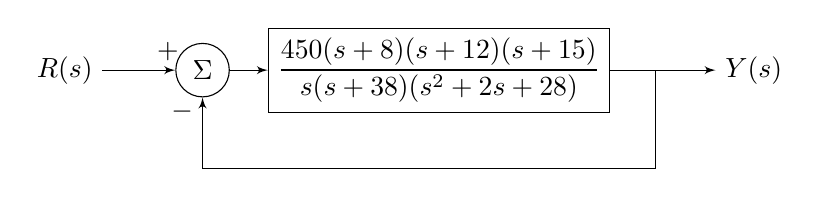
\begin{tikzpicture}[node distance=1.75cm,auto,>=latex']
	\node [input,align=center] (r) {$ R(s) $};
	\node [sum] (sumr) [right of=r] {$\Sigma$};
	\node [block] (gc) [right of=sumr,node distance=3cm] {$ \dfrac{450(s+8)(s+12)(s+15)}{s(s+38)(s^2+2s+28)} $};
	\node [waypoint] (sumd) [right of=gc,node distance=2.75cm] {};
	\node [output,align=center] (y) [right of=sumd,node distance=1.25cm]{$ Y(s) $};
	\node [waypoint] (h) [below of=gc,node distance=1.25cm] {};
	
	\draw[->] (r) -- node[pos=0.9] {$+$} (sumr);
	\draw[->] (sumr) -- (gc);
	\draw[->] (gc) -- (y);
	\draw[->] (sumd) |- (h)-| node[pos=0.9] {$-$} (sumr);
	\end{tikzpicture}
\end{center}
Find $ e_{ss} $ for:
\begin{itemize}
	\item[a)] $ r(t)=25\cdot1(t) $
	\item[b)] $ r(t)=37t\cdot1(t) $
	\item[c)] $ r(t)=(47/2)t^2\cdot1(t) $
\end{itemize}

This is a Type 1 unity feedback system ($ p=1 $). So, we can format $ L(s) $ as
\[ L(s) = \frac{K(b_3s^3 + b_{2}s^{2} +b_1s+1)}{s^1(a_3s^3 + a_{2}s^{2} +a_1s+1)} = \frac{Kb(s)}{s^1a(s)} \]
Then,
\begin{align*}
K_p &= \lim_{s\to0}L(s) = \infty \\
K_v &= \lim_{s\to0}sL(s) = \frac{450(8)(12)(15)}{38(28)} \approx 609.2\\
K_a &= \lim_{s\to0}s^2L(s) = 0
\end{align*}
So,
\begin{itemize}
	\item[a)] Step input $ \therefore e_{ss}=25\cdot\frac{1}{1+K_p}=0$ (remember the input magnitude is 25!)
	\item[b)] Ramp input: Error for a unit ramp is $ 1/K_v = 0.001642 $. So for a ramp with magnitude of 37, we have $ e_{ss}=37/K_v = 0.06075 $
	\item[c)] Parabolic input $ \therefore e_{ss}=\frac{47}{K_a}=\infty$
\end{itemize}

\paragraph*{Note!} All of the above is only valid for a \textbf{unity feedback system}. If we do not have unity feedback, we will need to approach the system in a different way. First, we must make an important distinction between \textbf{measured error} and \textbf{true error}. Consider the block diagram shown below. We must do this if our sensor dynamics are not fast enough.
\begin{center}
	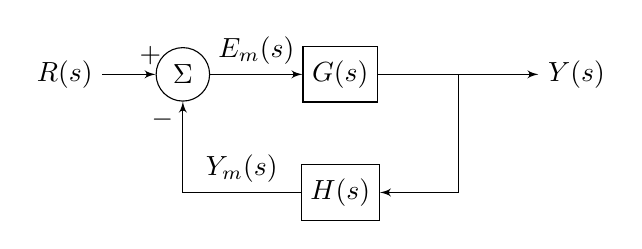
\begin{tikzpicture}[node distance=1.5cm,auto,>=latex']
	\node [input,align=center] (r) {$ R(s) $};
	\node [sum] (sumr) [right of=r] {$\Sigma$};
	\node [block] (gc) [right of=sumr,node distance=2cm] {$ G(s) $};
	\node [waypoint] (sumd) [right of=gc] {};
	\node [output,align=center] (y) [right of=sumd]{$ Y(s) $};
	\node [block] (h) [below of=gc] {$ H(s) $};
	
	\draw[->] (r) -- node[pos=0.9] {$+$} (sumr);
	\draw[->] (sumr) -- node[above]{$ E_m(s) $} (gc);
	\draw[->] (gc) -- (y);
	\draw[->] (sumd) |- (h);
	\draw[->] (h) -| node[above,pos=0.25] {$ Y_m(s) $} node[pos=0.9] {$-$} (sumr);
	\end{tikzpicture}
\end{center}
We can see that there is an output signal $ Y(s) $ that represents the true output of the system. That true output is measured by the sensor with dynamics $ H(s) $, resulting the measured output $ Y_m(s) $. Then, out system takes and error measurement of $ E_m(s) = R(s) - Y(s) $ to get the \textbf{measured error} $ E_m(s) $. However, unless we have $ H(s) = 1 $ (unity feedback), the measured output will be different from the true output, i.e. $ Y_m(s) \neq Y(s) $ and $ y_m(t) \neq y(t) $. We can denote a \textbf{true error} that represents the difference between the input (desired value) $ R(s) $ and true output $ Y(s) $ as $ E(s) = R(s) - Y(s) $.

There is value in looking at both the measured error and true error. The actual details of when measured vs. true error will be considered will be discussed later in the course; for now, we will only show how to obtain results for either case. There are two ways of proceeding:
\begin{enumerate}
	\item Use definition + final value theorem. In other words, find an expression for $ E(s) = R(s) - Y(s) $ or $ E_m(s) = R(s) - Y_m(s) $, verify it has a final value, and then apply the FVT.
	\item Convert the system to an equivalent unity-feedback system.
	% \item Assume the system behaves like a unity-feedback system. 
\end{enumerate}

\subsubsection*{Method 1}
For this method, we obtain direct expressions for the error by following the signals on the block diagram.

For measured error and following the signals shown in the above figure, we have
\begin{align*}
	E_m(s) &= R(s) - Y_m(s) \\
	&= R(s) - HY(s) \\
	&= R(s) - GHE_m(s) \\
	E_m(s)\big(1+GH\big)&=R(s) \\
	\Rightarrow E_m(s) &= \frac{1}{1+GH}R(s) 
\end{align*}
So for a given $ G(s) $, $ H(s) $, and $ R(s) $, the measured steady-state error can be obtained from the FVT using this expression of $ E_m(s) $.

Finding an expression for \textbf{true} steady-state error is a bit more complex. First we must obtain an expression for the true output $ Y(s) $ in terms of the input $ R(s) $.
\begin{align*}
Y(s) &= G E_m(s) \\
&= G\big(R(s) - Y_m(s)\big) \\
&= G\big(R(s) - HY(s)\big) \\
Y(s)\big(1+GH\big)&=GR(s) \\
\Rightarrow Y(s) &= \frac{G}{1+GH}R(s) 
\end{align*}
We can then substitute this definition into our expression for the true error:
\begin{align*}
E(s) &= R(s) - Y(s) \\
&= R(s) - \frac{G}{1+GH}R(s)  \\
&= \left(\frac{1+GH}{1+GH} - \frac{G}{1+GH} \right)R(s) \\
\Rightarrow E(s) &= \frac{1+GH-G}{1+GH}R(s) 
\end{align*}
For a given $ G(s) $, $ H(s) $, and $ R(s) $, the true steady-state error can be obtained from the FVT using this expression of $ E(s) $. Notice that in the case of unity feedback ($ H=1 $), the expressions for measured and true error turn out to be identical.

\subsubsection*{Method 2}
Finding the \textbf{measured} error for a non-unity feedback system requires little extra care. For measured steady-state error, we can simply use the return ratio $ L(s) = G(s)H(s) $ as-is in the above formulas for system type. 

However, \textbf{true} steady-state error for a non-unity feedback system takes more effort. In this method, we are going to transform a non-unity feedback system (left) into an equivalent unity feedback system (right). We will show this derivation using both algebra and block diagram manipulation.
\begin{center}
	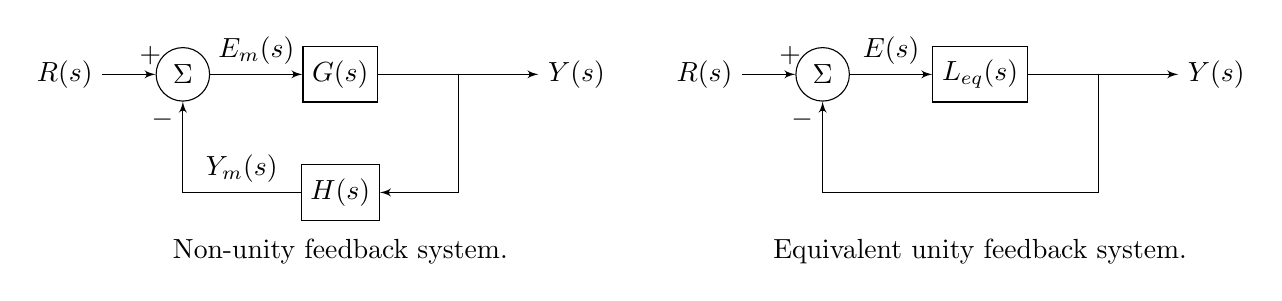
\begin{tikzpicture}[node distance=1.5cm,auto,>=latex']
	\begin{scope}
		\node [input,align=center] (r) {$ R(s) $};
		\node [sum] (sumr) [right of=r] {$\Sigma$};
		\node [block] (gc) [right of=sumr,node distance=2cm] {$ G(s) $};
		\node [waypoint] (sumd) [right of=gc] {};
		\node [output,align=center] (y) [right of=sumd]{$ Y(s) $};
		\node [block] (h) [below of=gc] {$ H(s) $};
		
		\draw[->] (r) -- node[pos=0.9] {$+$} (sumr);
		\draw[->] (sumr) -- node[above]{$ E_m(s) $} (gc);
		\draw[->] (gc) -- (y);
		\draw[->] (sumd) |- (h);
		\draw[->] (h) -| node[above,pos=0.25] {$ Y_m(s) $} node[pos=0.9] {$-$} (sumr);
		\node[below of=h,node distance=0.75cm] {Non-unity feedback system.};
	\end{scope}
	
	\begin{scope}[xshift=8.125cm]
		\node [input,align=center] (r) {$ R(s) $};
		\node [sum] (sumr) [right of=r] {$\Sigma$};
		\node [block] (gc) [right of=sumr,node distance=2cm] {$ L_{eq}(s) $};
		\node [waypoint] (sumd) [right of=gc] {};
		\node [output,align=center] (y) [right of=sumd]{$ Y(s) $};
		\node [waypoint] (h) [below of=gc] {};
		
		\draw[->] (r) -- node[pos=0.9] {$+$} (sumr);
		\draw[->] (sumr) -- node[above]{$ E(s) $} (gc);
		\draw[->] (gc) -- (y);
		\draw (sumd) |- (h);
		\draw[->] (h) -| node[pos=0.9] {$-$} (sumr);
		\node[below of=h,node distance=0.75cm] {Equivalent unity feedback system.};
	\end{scope}
	\end{tikzpicture}
\end{center}
Let's start by comparing the closed-loop transfer functions for these two systems.
\begin{center}
	\hfill
	\begin{minipage}{0.45\textwidth}
		\centering
		Non-unity feedback system
		\begin{align*}
		Y(s) &= G E_m(s) \\
		Y(s) &= G(R(s)-HY(s))\\
		Y(s) + GHY(s) &= GR(s)\\
		Y(s)(1+GH) &= GR(s)\\
		\Rightarrow\quad\frac{Y(s)}{R(s)} &= \frac{G}{1+GH}
		\end{align*}
	\end{minipage}
	\hfill
	\begin{minipage}{0.45\textwidth}
		\centering
		Unity feedback system
		\begin{align*}
		Y(s) &= L_{eq} E(s) \\
		Y(s) &= L_{eq}(R(s)-Y(s))\\
		Y(s) + L_{eq}Y(s) &= L_{eq}R(s)\\
		Y(s)(1+L_{eq}) &= L_{eq}R(s)\\
		\Rightarrow\quad\frac{Y(s)}{R(s)} &= \frac{L_{eq}}{1+L_{eq}}
		\end{align*}
	\end{minipage}
\hfill
\end{center}
We are looking for the $ L_{eq}(s) $ transfer function that makes the unity feedback system equivalent to the non-unity feedback system. If the systems are equivalent then they have the same closed-loop response. So,
\begin{align*}
	\frac{G}{1+GH} &= \frac{L_{eq}}{1+L_{eq}} \\
	(1+GH)L_{eq} &= G(1+L_{eq}) \\
	L_{eq} + LGH &= G + L_{eq}G \\
	G &= L_{eq} + L_{eq}GH - L_{eq}G \\
	G &= L_{eq}(1 + GH - G) \\
	\Rightarrow\quad L_{eq}(s) &= \frac{G(s)}{1 + G(s)H(s) - G(s)}
\end{align*}
Then, we can use the obtained $ L_{eq}(s) $ to compute the \textbf{true} steady-state error by finding $ K_p $, $ K_v $, $ K_a $, and so on using $ L_{eq}(s) $. The above formula can be used for any problem that has non-unity feedback.

Let's now look at repeating this derivation using block diagrams. Instead of using strictly algebra, we will use block diagram manipulations.
\begin{center}
\begin{minipage}{0.65\textwidth}
	\centering
	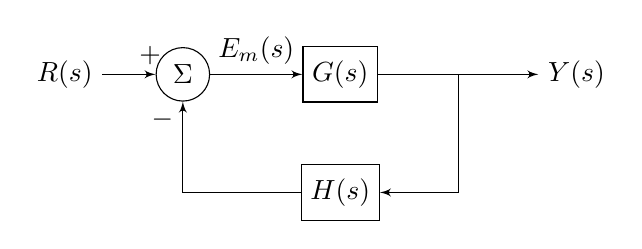
\begin{tikzpicture}[node distance=1.5cm,auto,>=latex',scale=0.96]
	\node [input,align=center] (r) {$ R(s) $};
	\node [sum] (sumr) [right of=r] {$\Sigma$};
	\node [block] (gc) [right of=sumr,node distance=2cm] {$ G(s) $};
	\node [waypoint] (sumd) [right of=gc] {};
	\node [output,align=center] (y) [right of=sumd]{$ Y(s) $};
	\node [block] (h) [below of=gc] {$ H(s) $};
	
	\draw[->] (r) -- node[pos=0.9] {$+$} (sumr);
	\draw[->] (sumr) -- node[above]{$ E_{m}(s) $} (gc);
	\draw[->] (gc) -- (y);
	\draw[->] (sumd) |- (h);
	\draw[->] (h) -| node[pos=0.9] {$-$} (sumr);
	
	\end{tikzpicture}
	
	\vspace{3em}
	
	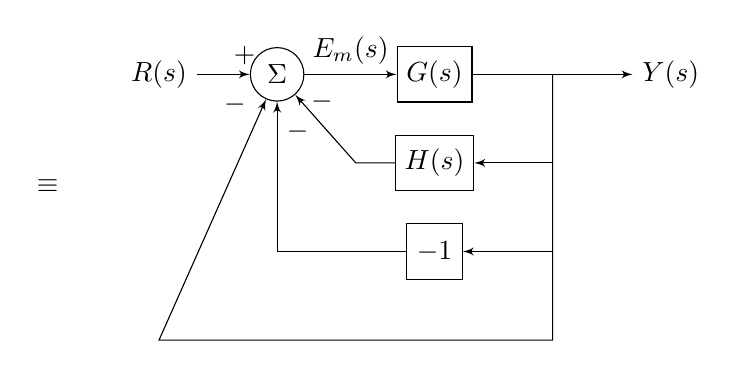
\begin{tikzpicture}[node distance=1.5cm,auto,>=latex',scale=0.96]
	\begin{scope}[shift={(9cm,0cm)}]
	\node [input,align=center] (r) {$ R(s) $};
	\node [sum] (sumr) [right of=r] {$\Sigma$};
	\node [block] (gc) [right of=sumr,node distance=2cm] {$ G(s) $};
	\node [waypoint] (sumd) [right of=gc] {};
	\node [output,align=center] (y) [right of=sumd]{$ Y(s) $};
	\node [block] (h) [below of=gc,node distance=1.125cm] {$ H(s) $};
	\node [waypoint] (h3) [left of=h,node distance=1cm] {};
	\node [block] (h1) [below of=h,node distance=1.125cm] {$ -1 $};
	\node [waypoint] (h2) [below of=r,node distance=3.375cm] {};
	
	\draw[->] (r) -- node[pos=0.9] {$+$} (sumr);
	\draw[->] (sumr) -- node[above]{$ E_m(s) $} (gc);
	\draw[->] (gc) -- (y);
	\draw[->] (sumd) |- (h);
	\draw[->] (h) -- (h3) -- node[pos=0.9,right] {$-$} (sumr);
	\draw[->] (sumd) |- (h1);
	\draw[->] (h1)-| node[pos=0.9,right] {$-$} (sumr);
	\draw[->] (sumd) |- (h2) -- node[pos=0.9] {$-$} (sumr);
	
	\node [below left of=r,node distance=2cm]{$ \equiv $};
	\end{scope}	
	\end{tikzpicture}
	
	\vspace{3em}
	
	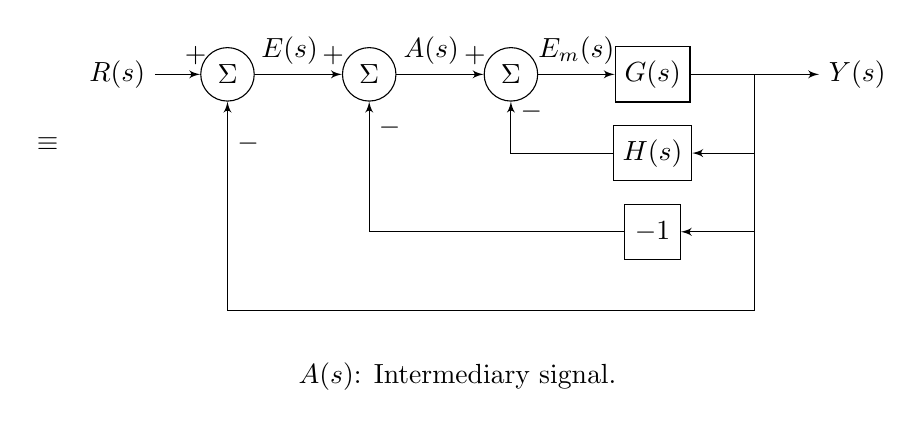
\begin{tikzpicture}[node distance=1.5cm,auto,>=latex',scale=0.96]
	\node [input,align=center] (r) {$ R(s) $};
	\node [sum] (sumr1) [right of=r,node distance=1.4cm] {$\Sigma$};
	\node [sum] (sumr2) [right of=sumr1,node distance=1.8cm] {$\Sigma$};
	\node [sum] (sumr) [right of=sumr2,node distance=1.8cm] {$\Sigma$};
	\node [block] (gc) [right of=sumr,node distance=1.8cm] {$ G(s) $};
	\node [waypoint] (sumd) [right of=gc,node distance=1.3cm] {};
	\node [output,align=center] (y) [right of=sumd,node distance=1.3cm]{$ Y(s) $};
	\node [block] (h) [below of=gc,node distance=1cm] {$ H(s) $};
	\node [block] (h1) [below of=h,node distance=1cm] {$ -1 $};
	\node [waypoint] (h2) [below of=h1,node distance=1cm] {};
	
	\draw[->] (r) -- node[pos=0.9] {$+$} (sumr1);
	\draw[->] (sumr1) -- node[above,pos=0.4]{$ E(s) $} node[pos=0.9] {$+$} (sumr2);
	\draw[->] (sumr2) -- node[above,pos=0.4]{$ A(s) $} node[pos=0.9] {$+$} (sumr);
	\draw[->] (sumr) -- node[above]{$ E_m(s) $} (gc);
	\draw[->] (gc) -- (y);
	\draw[->] (sumd) |- (h);
	\draw[->] (h) -| node[pos=0.9,right] {$-$} (sumr);
	\draw[->] (sumd) |- (h1);
	\draw[->] (h1) -| node[pos=0.9,right] {$-$} (sumr2);
	\draw[->] (sumd) |- (h2) -| node[pos=0.9,right] {$-$} (sumr1);
	
	\node [below left of=r,node distance=1.25cm]{$ \equiv $};
	\node at (4.5cm, -4cm) {$ A(s) $: Intermediary signal.};
	\end{tikzpicture}
\end{minipage}
\hfill
\begin{minipage}{0.3125\textwidth}
	\vspace{3em}
	
	Starting point. 
	
	\vspace{7.25em}
	
	Add $ Y(s) $ and $ -Y(s) $ to the summing junction:
	\[ E_m(s) = R(s) - HY(s) \]
	\[ \Downarrow \]
	\[ E_m(s) = R(s) - HY(s) + Y(s) - Y(s) \]
	The two new terms cancel, so the overall system stays the same.
	
	\vspace{2.75em}
	
	Split the summing junction apart.
	\[ E_m(s) = R(s) - HY(s) + Y(s) - Y(s) \]
	\[ \Downarrow \]
	\[ E_m(s) = \big((R(s) - HY(s)) + Y(s)\big) - Y(s) \]
	Addition is commutative, so the overall system remains the same.
	
	\vspace{3em}
\end{minipage}
\end{center}

\clearpage

\begin{center}
	\begin{minipage}{0.6\textwidth}
		\centering	
		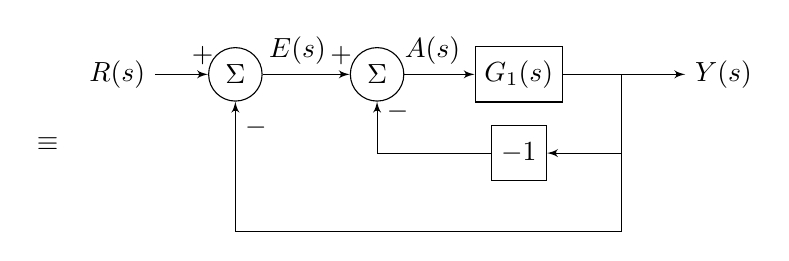
\begin{tikzpicture}[node distance=1.5cm,auto,>=latex',scale=0.96]
		\node [input,align=center] (r) {$ R(s) $};
		\node [sum] (sumr1) [right of=r] {$\Sigma$};
		\node [sum] (sumr2) [right of=sumr1,node distance=1.8cm] {$\Sigma$};
		\node [block] (gc) [right of=sumr2,node distance=1.8cm] {$ G_1(s) $};
		\node [waypoint] (sumd) [right of=gc,node distance=1.3cm] {};
		\node [output,align=center] (y) [right of=sumd,node distance=1.3cm]{$ Y(s) $};
		\node [block] (h1) [below of=gc,node distance=1cm] {$ -1 $};
		\node [waypoint] (h2) [below of=h1,node distance=1cm] {};
		
		\draw[->] (r) -- node[pos=0.9] {$+$} (sumr1);
		\draw[->] (sumr1) -- node[above,pos=0.4]{$ E(s) $} node[pos=0.9] {$+$} (sumr2);
		\draw[->] (sumr2) -- node[above,pos=0.4]{$ A(s) $} (gc);
		\draw[->] (gc) -- (y);
		\draw[->] (sumd) |- (h1);
		\draw[->] (h1) -| node[pos=0.9,right] {$-$} (sumr2);
		\draw[->] (sumd) |- (h2) -| node[pos=0.9,right] {$-$} (sumr1);
		
		\node [below left of=r,node distance=1.25cm]{$ \equiv $};
		\end{tikzpicture}
		
		\vspace{4em}
		
		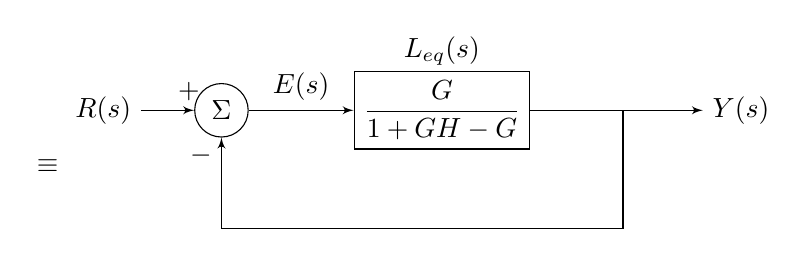
\begin{tikzpicture}[node distance=1.5cm,auto,>=latex',scale=0.96]
		\node [input,align=center] (r) {$ R(s) $};
		\node [sum] (sumr) [right of=r] {$\Sigma$};
		\node [block] (gc) [right of=sumr,node distance=2.8cm] {$ \dfrac{G}{1+GH-G} $};
		\node [waypoint] (sumd) [right of=gc,node distance=2.3cm] {};
		\node [output,align=center] (y) [right of=sumd]{$ Y(s) $};
		\node [waypoint] (h) [below of=gc] {};
		
		\draw[->] (r) -- node[pos=0.9] {$+$} (sumr);
		\draw[->] (sumr) -- node[above]{$ E(s) $} (gc);
		\draw[->] (gc) -- (y);
		\draw[->] (sumd) |- (h) -| node[pos=0.9] {$-$} (sumr);
		
		\node [below left of=r,node distance=1cm]{$ \equiv $};
		\node [above of=gc, node distance=0.75cm] {$ L_{eq}(s) $};
		\end{tikzpicture}
		
		\vspace{3em}
	\end{minipage}
	\hfill
	\begin{minipage}{0.35\textwidth}
		Close the $ H(s) $ feedback loop first:
		\begin{align*}
		Y(s) &= GE_m(s) \\
		Y(s) &= G(A(s)-HY(s)) \\ 
		Y(s)(1+H) &= G A(s) \\
		\Rightarrow G_1(s) \equiv \frac{Y(s)}{A(s)} &= \frac{G}{1+GH}
		\end{align*}
		
		\vspace{1.5em}
		
		Close the $ (-1) $ feedback loop next:
		\begin{align*}
		Y(s) &= G_1A(s) \\
		Y(s) &= G_1(E(s)+Y(s)) \\ 
		Y(s)(1-G_1) &= G_1 E(s) \\
		\Rightarrow L_{eq}(s) \equiv \frac{Y(s)}{E(s)} &= \frac{G_1}{1-G_1}
		\end{align*}
		
		\vspace{0.5em}
		
	\end{minipage}
\end{center}
Substituting in the definition of $ G(s) $ then gives:
\[ L_{eq}(s) = \frac{G_1}{1-G_1} = \frac{\dfrac{G}{1+GH}}{1-\dfrac{G}{1+GH}} = \frac{G}{1 + GH - G} \]
which matches the definition obtained earlier. 

%\vspace{1em}\noindent
%\textbf{Note:} We will cover block diagram manipulation in more depth in coming lectures.

\vspace{1em}
Note that for finding the \textbf{true} steady-state error for a non-unity feedback system, system type is not determined using the return ratio from the initial block diagram ($ L=GH $), but rather the equivalent return ratio from the final one ($ L_{eq} = G/(1+GH-G) $).

For \textbf{measured} error, the easiest approach is simply to find the closed-loop transfer function for the error signal and apply the FVT:
\[ \textrm{Closed-loop transfer function} = \frac{\textrm{Feedforward path TF}}{1 + \textrm{Return ratio TF}} \]
\[ \Rightarrow \frac{E_m(s)}{R(s)} = \frac{1}{1+GH} \]

\exmp
Find both the \textbf{true} and \textbf{measured} steady-state errors of the system, using both methods of dealing with non-unity feedback.
\begin{center}
	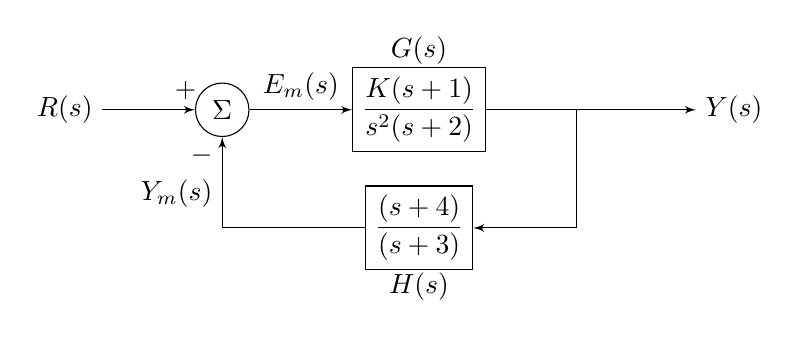
\begin{tikzpicture}[node distance=2.0cm,auto,>=latex']
	\node [input,align=center] (r) {$ R(s) $};
	\node [sum] (sumr) [right of=r] {$\Sigma$};
	\node [block] (gc) [right of=sumr,node distance=2.5cm] {$ \dfrac{K(s+1)}{s^2(s+2)} $};
	\node [waypoint] (sumd) [right of=gc] {};
	\node [output,align=center] (y) [right of=sumd]{$ Y(s) $};
	\node [block] (h) [below of=gc,node distance=1.5cm] {$ \dfrac{(s+4)}{(s+3)} $};
	
	\draw[->] (r) -- node[pos=0.9] {$+$} (sumr);
	\draw[->] (sumr) -- node {$E_m(s)$} (gc);
	\draw[->] (gc) -- (y);
	\draw[->] (sumd) |- (h);
	\draw[->] (h) -| node[left, pos=0.6875] {$Y_m(s)$} node[pos=0.9] {$-$} (sumr);	
	
	\node[above of=gc,node distance=0.75cm] {$ G(s) $};
	\node[below of=h,node distance=0.75cm] {$ H(s) $};
	\end{tikzpicture}
\end{center}
\subsubsection*{Method 1}
\paragraph*{Measured Error}  Using the derivation given earlier, we have an expression for the true error as
\begin{align*}
E_m(s) &= R(s) - Y_m(s) \\
&= \frac{1}{1+GH}R(s) \\
&= \frac{1}{1+\dfrac{K(s+1)(s+4)}{s^2(s+2)(s+3)}} R(s) \\
\Rightarrow E_m(s) &= \frac{s^2(s+2)(s+3)}{s^2(s+2)(s+3)+K(s+1)(s+4)} R(s)
\end{align*}
The final value theorem can then be used on this expression of $ E_m(s) $. 

\noindent For a step input $ R(s) = 1/s $:
\[ e_{ss,meas} = \lim_{s\to0} sE_m(s) = \lim_{s\to0} s\cdot\frac{1}{s} \cdot \frac{s^2(s+2)(s+3)}{s^2(s+2)(s+3)+K(s+1)(s+4)} = 0  \]
For a ramp input $ R(s) = 1/s^2 $:
\[ e_{ss,meas} = \lim_{s\to0} sE_m(s) = \lim_{s\to0} s\cdot\frac{1}{s^2} \cdot \frac{s^2(s+2)(s+3)}{s^2(s+2)(s+3)+K(s+1)(s+4)} = 0  \]
For a parabolic input $ R(s) = 2/s^3 $:
\[ e_{ss,meas} = \lim_{s\to0} sE_m(s) = \lim_{s\to0} s\cdot\frac{2}{s^3} \cdot \frac{s^2(s+2)(s+3)}{s^2(s+2)(s+3)+K(s+1)(s+4)} = \frac{2\cdot2\cdot3}{0+K\cdot1\cdot4} = \frac{3}{K}  \]
For a cubic input $ R(s) = 6/s^4 $:
\[ e_{ss,meas} = \lim_{s\to0} sE_m(s) = \lim_{s\to0} s\cdot\frac{6}{s^4} \cdot \frac{s^2(s+2)(s+3)}{s^2(s+2)(s+3)+K(s+1)(s+4)} = \infty  \]
So, we have $ e_{ss,meas} = 3/K $ for parabolic inputs, and $ e_{ss,meas} = 0 $ for lower-order inputs and $  e_{ss,meas}\to\infty $ for higher-order inputs (such as cubic, etc...).

\paragraph*{True Error} Using the derivation given earlier, we have an expression for the true error as
\begin{align*}
E(s) &= R(s) - Y(s) \\
&= \frac{1+GH-G}{1+GH}R(s) \\
&= \frac{1+\dfrac{K(s+1)(s+4)}{s^2(s+2)(s+3)}-\dfrac{K(s+1)}{s^2(s+2)}}{1+\dfrac{K(s+1)(s+4)}{s^2(s+2)(s+3)}} R(s) \\
&= \frac{ s^2(s+2)(s+3) + K(s+1)(s+4) - K(s+1)(s+3) }{ s^2(s+2)(s+3) + K(s+1)(s+4) } R(s) \\
\Rightarrow E(s) &= \frac{ s^2(s+2)(s+3) + K(s+1) }{ s^2(s+2)(s+3) + K(s+1)(s+4) } R(s)
\end{align*}
The final value theorem can then be used on this expression of $ E(s) $.

\noindent For a step input $ R(s) = 1/s $:
\[ e_{ss,true} = \lim_{s\to0} sE(s) = \lim_{s\to0} s\cdot\frac{1}{s}\cdot \frac{s^2(s+2)(s+3)+K(s+1)}{s^2(s+2)(s+3)+K(s+1)(s+4)} = \frac{K}{K(1)(4)} = \frac{1}{4} \]
For a ramp input $ R(s) = 1/s^2 $:
\[ e_{ss,true} = \lim_{s\to0} sE(s) = \lim_{s\to0} s\cdot\frac{1}{s^2}\cdot \frac{s^2(s+2)(s+3)+K(s+1)}{s^2(s+2)(s+3)+K(s+1)(s+4)} = \infty \]
So, we have $ e_{ss,true} = 1/4 $ for step inputs and $ e_{ss,true}\to\infty $ for larger inputs (such as ramps, parabolas, etc...).

\subsubsection*{Method 2 - Formula}
\paragraph*{Measured Error} For steady-state \textbf{measured} error, we can use the regular formulas for system type. So, we have
\[ L(s) = G(s)H(s) = \frac{K(s+1)(s+4)}{s^2(s+3)(s+2)} \]
This is a \textbf{Type 2} system. So that means:
\begin{itemize}
	\item For a step input $\frac{1}{s} $:
	\[ K_p = \lim_{s\to 0} L(s) = \infty \quad\Rightarrow\quad e_{ss,meas} = \frac{1}{1+K_p} = 0 \]
	\item For a ramp input $ \frac{1}{s^2} $:
	\[ K_v = \lim_{s\to 0} sL(s) = \infty \quad\Rightarrow\quad e_{ss,meas} = \frac{1}{K_v} = 0 \]
	\item For a parabolic input $ \frac{1}{s^3} $:
	\[ K_a = \lim_{s\to 0} s^2L(s) = \frac{2K}{3} \quad\Rightarrow\quad e_{ss,meas} = \frac{1}{K_a} = \frac{3}{2K} \]
	However, a \textbf{unit} parabola $ r(t) = t^3 $ is $ R(s) = \frac{\mathbf{2}}{s^3} $, so for a \textbf{unit} parabola we have $ e_{ss,meas} = \frac{3}{K} $, in line with earlier results.
	\item For a cubic input  $ \frac{1}{s^4} $:
	\[ K_c = \lim_{s\to 0} s^3L(s) = 0 \quad\Rightarrow\quad e_{ss,meas} = \frac{1}{K_c} = \infty \]
\end{itemize}
Clearly, this method matches what was obtained using the FVT in Method 1.

\paragraph*{True Error} 
Start by finding the equivalent unity-feedback return ratio. 
\[ L_{eq}(s) = \frac{G(s)}{1 + G(s)H(s) - G(s)} \]
\[ G(s) = \frac{K(s+1)}{s^2(s+2)},\quad H(s) = \frac{s+4}{s+3} \]
Substitute in:
\[ L_{eq}(s) = \frac{\dfrac{K(s+1)}{s^2(s+2)}}{1 + \dfrac{K(s+1)}{s^2(s+2)}\times \dfrac{s+4}{s+3} - \dfrac{K(s+1)}{s^2(s+2)}} \]
Simplify:
\begin{align*}
L_{eq}(s) &= \frac { K(s+1)(s+3) }{ s^2(s+2)(s+3) + K(s+1)(s+4) - K(s+1)(s+3) }\\
&= \dfrac{K(s^2+4s+3)}{s^4+5s^3+6s^2+Ks+K} 
\end{align*}
We look at the denominator to tell what type of system this is: There are no poles at the origin, so this is a Type 0 system. So,
\[ K_p = \lim_{s\to0}L_{eq}(s)=\frac{K(3)}{K} = 3 \]
and
\[ e_{ss,true} = \frac{1}{1+K_p} = \frac{1}{1+3} = \frac{1}{4} \]
for step inputs and is infinite for ramps, parabolas, and so on. This matches the results we found using the first method.


\subsubsection*{Method 2 - Block Diagram Manipulation - True error only}
Using the formula, as above, is sufficient for any non-unity feedback problem. For the sake of example, we can also show how to obtain this using block diagram manipulation. First, we modify the system so that we have unity feedback:
\begin{center}
	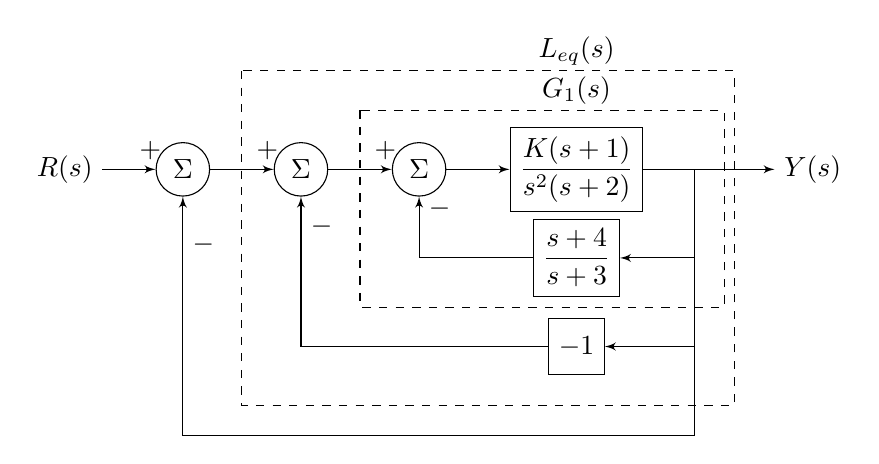
\begin{tikzpicture}[node distance=1.5cm,auto,>=latex']
	\node [input,align=center] (r) {$ R(s) $};
	\node [sum] (sumr1) [right of=r] {$\Sigma$};
	\node [sum] (sumr2) [right of=sumr1] {$\Sigma$};
	\node [sum] (sumr) [right of=sumr2] {$\Sigma$};
	\node [block] (gc) [right of=sumr,node distance=2cm] {$ \dfrac{K(s+1)}{s^2(s+2)}$};
	\node [waypoint] (sumd) [right of=gc] {};
	\node [output,align=center] (y) [right of=sumd]{$ Y(s) $};
	\node [block] (h) [below of=gc,node distance=1.125cm] {$ \dfrac{s+4}{s+3} $};
	\node [block] (h1) [below of=h,node distance=1.125cm] {$ -1 $};
	\node [waypoint] (h2) [below of=h1,node distance=1.125cm] {};
	
	\draw[->] (r) -- node[pos=0.9] {$+$} (sumr1);
	\draw[->] (sumr1) -- node[pos=0.9] {$+$} (sumr2);
	\draw[->] (sumr2) -- node[pos=0.9] {$+$} (sumr);
	\draw[->] (sumr) -- (gc);
	\draw[->] (gc) -- (y);
	\draw[->] (sumd) |- (h);
	\draw[->] (h) -| node[pos=0.9,right] {$-$} (sumr);
	\draw[->] (sumd) |- (h1);
	\draw[->] (h1) -| node[pos=0.9,right] {$-$} (sumr2);
	\draw[->] (sumd) |- (h2) -| node[pos=0.9,right] {$-$} (sumr1);
	
	\draw[dashed] (3.75cm,0.75cm) rectangle (8.375cm,-1.75cm);
	\draw[dashed] (2.25cm,1.25cm) rectangle (8.5cm,-3cm);
	
	\node[above of=gc,node distance = 1cm] {$ G_1(s) $};
	\node[above of=gc,node distance = 1.5cm] {$ L_{eq}(s) $};
	\end{tikzpicture}
\end{center}
Condense the innermost loop:
\[ G_1(s) = \frac{G(s)}{1+G(s)H(s)} = \dfrac{K(s+1)(s+3)}{s^2(s+2)(s+3) + K(s+1)(s+4)} \]
Condense the middle loop:
\begin{align*}
L_{eq}(s) = \dfrac{G_1}{1-G_1}& = \dfrac{\dfrac{K(s+1)(s+3)}{s^2(s+2)(s+3) + K(s+1)(s+4)}}{1-\dfrac{K(s+1)(s+3)}{s^2(s+2)(s+3) + K(s+1)(s+4)}}\\
& = \dfrac{K(s+1)(s+3)}{s^2(s+2)(s+3) + K(s+1)(s+4) - K(s+1)(s+3)}\\
& = \dfrac{K(s^2+4s+3)}{s^4+5s^3+6s^2+Ks+K} 
\end{align*}
Then, the steady-state error can be found from $ L_{eq}(s) $ as shown above.

\subsubsection*{Note:} If you mistakenly tried to find the steady-state error without accounting for the  non-unity feedback system, (that is, treated $ H $ as equal to $ 1 $, when that is not the case), and so defined $ L(s) $ as
\[ L(s) = \dfrac{K(s+1)}{s^2(s+2)} \]
You would have obtained incorrect results! Your \textbf{measured} error would have the correct system type, but would be off by a factor of 3 for the parabolic error. For \textbf{true} error, you would have misidentified the system as Type 2, with 0 steady-state error for step and ramp inputs.

\subsection*{Summary}
\begin{itemize}
	\item If system type is too low, some command signals will not be tracked.
	\item Decision about system type is probably one of the 1st things you want to do in the selection of a compensator.
		\begin{itemize}
			\item Add poles at the origin to increase system type to the appropriate value.
		\end{itemize}
	\item Never decrease system type! This could violate internal stability. The only way you can do this is to cancel unstable poles at the origin.
	\begin{itemize}
		\item (More on internal stability and canceling poles later.)
	\end{itemize}
		
\end{itemize}
\end{document}

